\documentclass[xcolor=dvipsnames,table]{beamer}

\usepackage{latexsym}
\usepackage[utf8]{inputenc}
\usepackage[brazil]{babel}
\usepackage{amssymb}
\usepackage{amsmath}
\usepackage{stmaryrd}
\usepackage{fancybox}
\usepackage{datetime}
\usepackage[T1]{fontenc}
\usepackage{graphicx}
\usepackage{graphics}
\usepackage{url}
\usepackage{algorithmic}
\usepackage{algorithm}
\usepackage{acronym}
\usepackage{array}

\newtheorem{definicao}{Definio}
\newcommand{\tab}{\hspace*{2em}}

\mode<presentation>
{
  \definecolor{colortexto}{RGB}{0,0,0}
 
  \setbeamertemplate{background canvas}[vertical shading][ bottom=white!10,top=white!10]
  \setbeamercolor{normal text}{fg=colortexto} 

  \usetheme{Warsaw}
}

\title{Definição de Algoritmo} 

\author{
  Esdras Lins Bispo Jr. \\ \url{bispojr@ufg.br}
  } 
 \institute{
  Teoria da Computação \\Bacharelado em Ciência da Computação}
\date{\textbf{10 de abril de 2018} }

\logo{
\includegraphics[width=1cm]{images/ufgJataiLogo.png}}

\begin{document}

	\begin{frame}
		\titlepage
	\end{frame}

	\AtBeginSection{
		\begin{frame}{Sumário}%[allowframebreaks]{Sumário}
    		\tableofcontents[currentsection]
    		%\tableofcontents[currentsection, hideothersubsections]
		\end{frame}
	}

	\begin{frame}{Plano de Aula}
		\tableofcontents
		%\tableofcontents[hideallsubsections]
	\end{frame}
	
	
%------------------------------------------
	\section{Revisão}
	
	\subsection{Máquina de Turing}
	\begin{frame}{Problema}
		\begin{block}{Problema 3.15 (a)}
			Mostre que a coleção de linguagens decidíveis é fechada sob a operação de união.		
		\end{block}  
		\begin{center}
			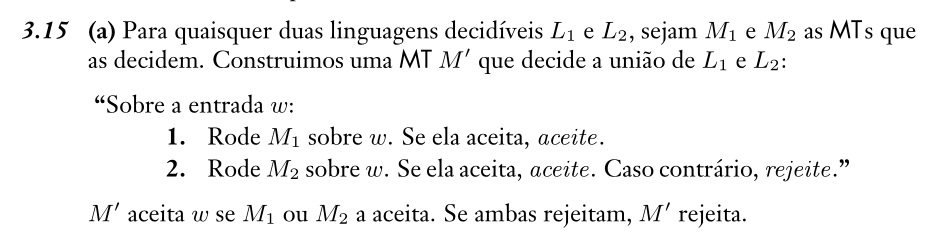
\includegraphics[height=2.7cm]{images/ex3-15a}
		\end{center}
	\end{frame}
	
	\subsection{Variantes da MT}
	\begin{frame}[shrink]{MT Multifita}
		\begin{block}{Definição}
			Uma {\bf máquina de Turing multifita} é como uma máquina de Turing comum com várias fitas:
			\begin{itemize}  
				\item cada fita tem sua própria cabeça de leitura e escrita;  
				\item a configuração inicial consiste da cadeia de entrada aparecer sobre a fita 1, e as outras iniciar em branco;  
				\item a função de transição permite ler, escrever e mover as cabeças em algumas ou em todas as fitas simultaneamente
				\begin{center}
					$\delta : Q \times \Gamma^k \rightarrow Q \times \Gamma^k \times \{E,D,P\}^k$
				\end{center}
				em que $k$ é o número de fitas.
			\end{itemize}
		\end{block} 
		\begin{block}{Exemplo}
			$\delta(q_i, a_1, \ldots, a_k) = (q_j, b_1, \ldots, b_k, P, D, \ldots, E)$
		\end{block}
	\end{frame}
	
	\begin{frame}{MT Multifita}
		\begin{block}{Teorema}
			Toda máquina de Turing multifita tem uma máquina de Turing de uma única fita que lhe é equivalente.
		\end{block}
	\end{frame}
	
	\begin{frame}{MT Multifita}
		\begin{center}
			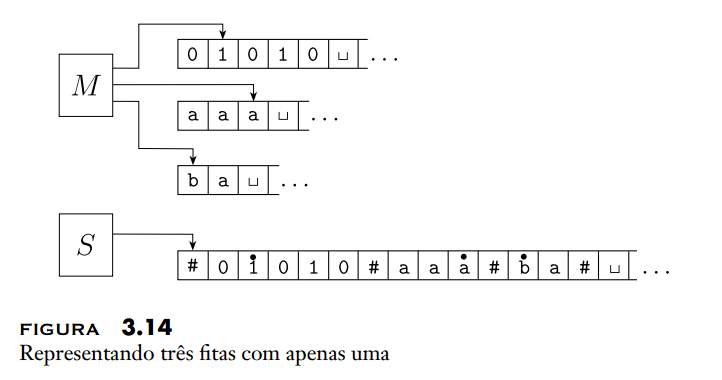
\includegraphics[height=6cm]{images/fig314.png}
		\end{center}
	\end{frame}
	
	\begin{frame}{MT Multifita}
		\begin{center}
			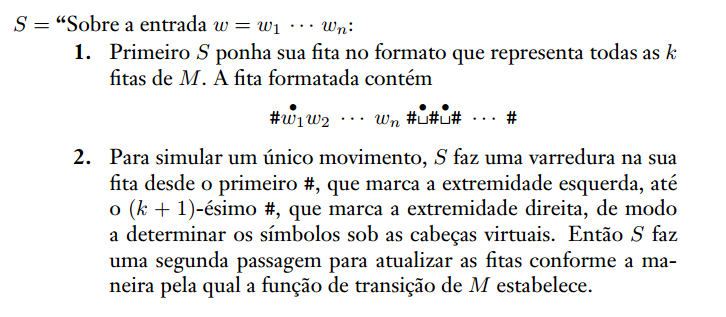
\includegraphics[height=5cm]{images/teoMt-1.png}
		\end{center}
	\end{frame}
	
	\begin{frame}{MT Multifita}
		\begin{center}
			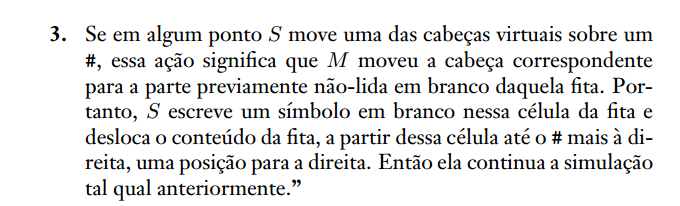
\includegraphics[height=3.3cm]{images/teoMt-2.png}
		\end{center}
	\end{frame}
	
	\begin{frame}{MT Multifita}
		\begin{block}{Teorema}
			Toda máquina de Turing multifita tem uma máquina de Turing de uma única fita que lhe é equivalente.
		\end{block}  
		\begin{block}{Corolário}
			Uma linguagem é Turing-reconhecível se e somente se alguma máquina de Turing multifita a reconhece.
		\end{block}
	\end{frame}
	
	\begin{frame}{MT Multifita}
		\begin{center}
			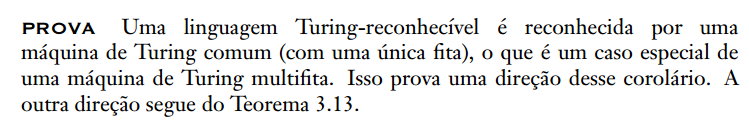
\includegraphics[height=1.8cm]{images/provaCorolario.png}
		\end{center}
	\end{frame}

	\section{Definição de algoritmo}
	\begin{frame}{Problema}
		\begin{block}{Problema 3.16 (b)}
			Mostre que a coleção de linguagens Turing-reconhecíveis é fechada sob a operação de concatenação.		
		\end{block}
	\end{frame}
	
	\begin{frame}{Problema} 
		
		{\bf Prova:} Sejam duas linguagens Turing-reconhecíveis (TR) quaisquer $A$ e $B$. \pause Sejam $M_A$ e $M_B$ as duas máquinas de Turing (MT) que reconhecem $A$ e $B$, respectivamente \pause (pois se uma linguagem é Turing-reconhecível, então uma MT a reconhece). \pause Iremos construir uma MT não-determinística (MTN) $M_{aux}$, a partir de $M_A$ e $M_B$, que reconhece $A \circ B$. \pause A descrição de $M_{aux}$ é dada a seguir: \pause
		
		$M_{aux}$ = ``Sobre a entrada $\omega$, faça: \pause
		\begin{enumerate}
			\item Corte, não deterministicamente, $\omega$ em duas cadeias \\(i.e. $\omega = \omega_1 \circ \omega_2$). \pause
			\item Rode $M_A$ sobre $\omega_1$. Se $M_A$ rejeita, {\it rejeite}. \pause
			\item Rode $M_B$ sobre $\omega_2$. Se $M_B$ aceita, {\it aceite}. \pause
			\item {\it Rejeite}''.
		\end{enumerate} \pause
		
		Como é possível construir $M_{aux}$, então $A \circ B$ é TR \pause (pois toda MTN tem uma MT equivalente). \pause Logo, a classe de linguagens Turing-reconhecíveis é fechada sob a operação de concatenação $\blacksquare$
	\end{frame}
	
	\begin{frame}{Definição de algoritmo}
		\begin{columns}
			\column{.4\textwidth}  		
			\begin{center}
				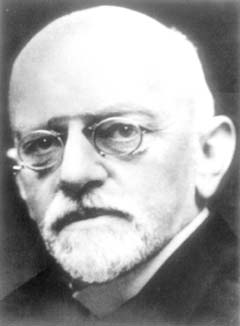
\includegraphics[height=.5\textheight]{images/hilbert.jpg}
			\end{center}
			\column{.6\textwidth}  		
			\begin{block}{Contribuição}
				\begin{center}
					{\large Apresentou uma noção do que seria um algoritmo no Congresso Internacional de Matemáticos em Paris, no ano de 1900.}
				\end{center}
			\end{block}		  		
			\begin{block}{Quem?}
				\begin{center}
					{\bf David Hilbert (1862-1943)} \\ Matemático alemão.
				\end{center}
			\end{block}
		\end{columns}
	\end{frame}
	
	\begin{frame}{Polinômio}
		\begin{block}{Definições}	
			Um {\bf polinômio} é uma soma de termos. Um {\bf termo} é um produto de variáveis e uma constante chamada de {\bf coeficiente}.
		\end{block}\pause
		\begin{block}{Exemplo: Termo}
			$6 \cdot x \cdot x \cdot y \cdot z \cdot z \cdot z= 6x^2 y z^3$
		\end{block}\pause
		\begin{block}{Exemplo: Polinômio}
			$6x^2 y z^3 + 3x y^2 - 10$
		\end{block}
	\end{frame}
	
	\begin{frame}{Polinômio}
		\begin{block}{Definições}	
			Uma {\bf raiz} de um polinômio é uma atribuição de valores às suas variáveis de modo que o valor do mesmo seja 0. Chamamos de {\bf raiz inteira} aquela em todos os valores atribuídos são valores inteiros.
		\end{block}\pause
		\begin{block}{Exemplo: Raiz}
			O polinômio $6x^3 y z^2 + 3x y^2 -x^3 - 10$ tem uma raiz em $x=5, y=3$ e $z=0$.
		\end{block}\pause
		\begin{block}{Exemplo: Raiz Inteira}
			A raiz do exemplo acima é uma raiz inteira.
		\end{block}
	\end{frame}
	
	\begin{frame}{Polinômio}
		\begin{block}{Problema apresentado por Hilbert}
			É possível conceber um algoritmo que teste se um polinômio tem uma raiz inteira ou não?
		\end{block} \pause
		\begin{block}{Expressão utilizada por Hilbert}
			``Um processo com o qual ela possa ser determinada por um número finito de operações''.
		\end{block} \pause
		\begin{alertblock}{Curioso}
			Não existe algoritmo que execute esta tarefa.
		\end{alertblock}
	\end{frame}
	
	\begin{frame}{Definição de algoritmo}
		\begin{columns}
			\column{.4\textwidth}  		
			\begin{center}
				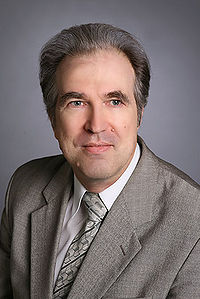
\includegraphics[height=.6\textheight]{images/yuri.jpg}
			\end{center}
			\column{.6\textwidth}  		
			\begin{block}{Contribuição}
				\begin{center}
					{\large Mostrou, em 1970, que não existe algoritmo para se testar se um polinômio tem raízes inteiras.}
				\end{center}
			\end{block}		  		
			\begin{block}{Quem?}
				\begin{center}
					{\bf Yuri Matijasevich (1947-)} \\ Cientista da computação e \\matemático russo.
				\end{center}
			\end{block}
		\end{columns}
	\end{frame}	
	
	\begin{frame}{Definição de Algoritmo}
		\begin{center}
			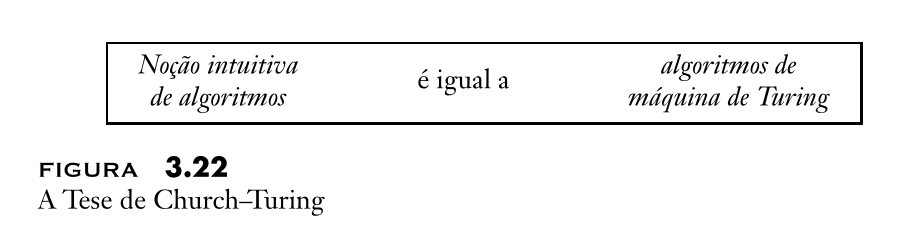
\includegraphics[width=11cm]{images/fig322.png}
		\end{center} \pause
		\begin{alertblock}{Conclusão}
			Existem problemas que são algoritmicamente insolúveis.
		\end{alertblock}
	\end{frame}
	
	\begin{frame}{Definição de Algoritmo}
		\begin{block}{Contexto}
			$D = \{ p \mbox{ | } p$ é um polinômio com uma raiz inteira$\}$
		\end{block} \pause
		\begin{block}{Problema}
			O conjunto $D$ é decidível?
		\end{block} \pause
		\begin{block}{Resposta}
			Não é decidível. Mas é Turing-reconhecível.
		\end{block}
	\end{frame}
	
	\begin{frame}{Definição de Algoritmo}
		\begin{block}{Problema análogo}
			$D_1 = \{p \mbox{ | } p$ é um polinômio sobre $x$ com uma raiz inteira$\}$
		\end{block} \pause
		\begin{block}{MT $M_1$ que reconhece $D_1$}
			$M_1$ = ``A entrada é um polinômio $p$ sobre a variável $x$.
			\begin{enumerate}
				\item Calcule o valor de $p$ com $x$ substituída sucessivamente pelos valores $0, 1,-1, 2, -2, 3, -3, \ldots$ \\Se em algum ponto o valor do polinômio resulta em $0$, {\it aceite}.
			\end{enumerate}
		\end{block}\pause
		\begin{block}{Considerações}
			$M_1$ reconhece $D_1$, mas não a decide.
		\end{block}
	\end{frame} 
	
	\begin{frame}[shrink]{Definição de Algoritmo}
		\begin{block}{Resultado obtido por Matijasevich}
			É possível construir um decisor para $D_1$. Mas não para $D$.
		\end{block} \pause
		\begin{block}{Justificativa}
			É possível obter um limitante para polinômios de uma única variável. Porém, Matijasevich provou ser impossível calcular tais limitantes para polinômios multivariáveis.
		\end{block}\pause
		\begin{block}{Limitante para polinômios de uma única variável}
			\begin{center}
				$\pm k \dfrac{c_{max}}{c_1}$
			\end{center}
			em que 
			\begin{itemize}
				\item $k$ é o número de termos do polinômio,
				\item $c_{max}$ é o coeficiente com maior valor absoluto, e
				\item $c_1$ é o coeficiente do termo de mais alta ordem.
			\end{itemize}  
		\end{block}
	\end{frame}
	
	\begin{frame}
		\titlepage
	\end{frame}
	
\end{document}